
\documentclass[11pt]{article}
\usepackage[utf8]{inputenc}
\usepackage[T1]{fontenc}
\usepackage{amssymb}
\usepackage{booktabs}
\usepackage{array}
\usepackage{filecontents}
\usepackage{pgfplotstable}
\pgfplotstableset{
  empty cells with={---},
  every head row/.style={before row=\toprule,after row=\midrule},
  every last row/.style={after row=\bottomrule}
}
\pgfplotsset{compat=1.9}

\begin{document}

\title{Inteligência Artificial - TP2\\Aprendizado por Reforço}
\author{Guilherme Torres\\Departamento de Ciência da Computação - UFMG}
\date{}
\maketitle

\section{Introdução}

O objetivo do trabalho que segue foi implementar um algoritmo de aprendizado por reforço, para encontrar a política ótima para um modelo de decisões de Markov em um ambiente parcialmente observável. Para isso, foi usado o algoritmo Q-learning[1], que faz passeios aleatórios nos estados e atualiza a função qualidade $Q(s, a)$ para cada um dos estados.

O programa recebe como entrada um mapa como uma matriz de caracteres e o agente pode se movimentar em quatro direções. Existem posições terminais (situações onde o agente termina de se movimentar) e não-terminais. Ao terminar, o programa produz como saída um arquivo \textit{q.txt} com as ações recomendadas e função qualidade para cada uma das posições não terminais, e \textit{pi.txt}, um mapa com as direções recomendadas pelo algoritmo em cada situação.

O programa foi implementado na linguagem Rust (rustc versão 1.21.0, cargo versão 0.22.0). O código fonte está na pasta src/. Para compilar, segue o script \textit{compila.sh} e o script \textit{qlearning.sh} compila e executa o programa, tendo como parâmetros, respectivamente, o mapa de entrada, a taxa de aprendizado $\alpha$, a taxa de desconto $\gamma$ e o número de iterações do algoritmo.

As decisões tomadas na implementação e o algoritmo estão explicitados na seção seguinte.

\section{Implementação e funcionamento}

\subsection{Algoritmo}

O algoritmo de Q-learning implementado pode ser descrito nos seguintes passos:

\begin{enumerate}
	\item É definido o valor inicial de $Q(s, a)$ para todas as ações $a$ e cada estado $s$ como zero
	\item A posição do agente é marcada como uma posição não-terminal aleatória no mapa.
	\item Uma ação aleatória é escolhida.
	\item O valor de $Q(s, a)$ para o estado atual e a ação escolhida é atualizado.
	\item O estado é atualizado.
	\item Se o estado atual for um terminal, define novamente uma posição não-terminal aleatória.
	\item Repete os itens 3 a 6 até atingir o número pré-definido de iterações.
	\item Produz os arquivos de saída.
\end{enumerate}

\subsection{Atualização da função Q(s, a)}

A função $Q(s, a)$ de um estado é atualizada segundo a equação:
$$Q(s, a) \leftarrow (1 - \alpha)Q(s, a) + \alpha(r(s')+\max_{a'} Q(s', a'))$$
sendo $\alpha$ a taxa de aprendizado, $\gamma$ a taxa de desconto do valor do próximo estado, $a$ a ação escolhida aleatoriamente, $s'$ o estado alcançado ao se executar a ação $a$ no estado $s$ e $max_{a'}$ a ação que tem o maior valor de $Q(s', a')$.

\subsection{Os valores $\alpha$ e $\gamma$}

Durante os testes, os parâmetros $\alpha$ e $\gamma$ foram mantidos estáticos a cada execução, ou seja, eles não se alteraram durante o curso do programa.

$\alpha$ teve o valor inicial de $0.2$, e esteve sujeito a variações entre os testes por ser um fator primordial no controle do \textit{Exploration vs. exploitation}. Basicamente, um valor mais alto nesse parâmetro indica que haverá uma convergência maior do programa às tendências que ele encontrar de início. Um valor menor abre espaço para mais exploração.

$\gamma$ também tém uma participação nesse aspecto do algoritmo, porém menor, por isso o seu valor durante os testes foi fixo em $0.9$.

\subsection{Número de iterações}

O número de iterações deve ser o suficiente para o programa apresentar uma convergência. Como foi implementado em Rust, uma linguagem compilada para arquivos binários, e, portanto, muito rápida, pôde-se dar ao luxo de fazer $100000$ iterações em tempo hábil. Porém, para que fosse posível notar a diferença da velocidade de convergência entre as diferentes taxas de aprendizado, os testes na seção seguinte foram feitos com $3000$ iterações, mas reforça-se que, a longo prazo, todas as taxas de aprendizado tendem a convergir para uma política em particular.

\section{Testes}

Os testes a seguir foram realizados em uma máquina com OS Linux Debian 9, processador Pentium G4400 dual-core (3.3Ghz) e 4x2 Gb de memória RAM. Todos eles rodaram em tempo hábil (menos de um segundo), com os parâmetros especificados acima. Os arquivos de teste podem ser encontrados na pasta maps/.

\subsection{pacmaze-01-tiny.txt}

Formato do teste:

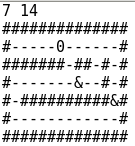
\includegraphics[scale=.5]{tst1map.png}

$\alpha = 0.2$

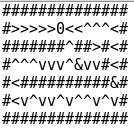
\includegraphics[scale=.5]{tst1-02.png}

$\alpha = 0.5$

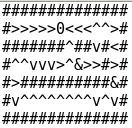
\includegraphics[scale=.5]{tst1-05.png}

$\alpha = 0.8$

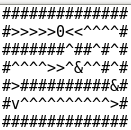
\includegraphics[scale=.5]{tst1-08.png}

$\alpha = 1.0$

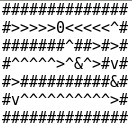
\includegraphics[scale=.5]{tst1-10.png}

\subsection{pacmaze-02-mid-sparse.txt}

Formato do teste:

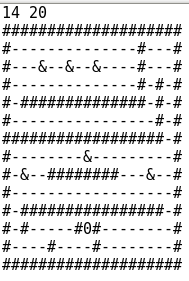
\includegraphics[scale=.5]{tst2-map.png}

$\alpha = 0.2$

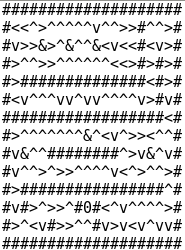
\includegraphics[scale=.5]{tst2-02.png}

$\alpha = 0.5$

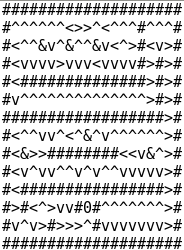
\includegraphics[scale=.5]{tst2-05.png}

$\alpha = 0.8$

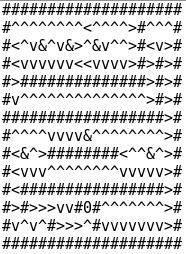
\includegraphics[scale=.5]{tst2-08.png}

$\alpha = 1.0$

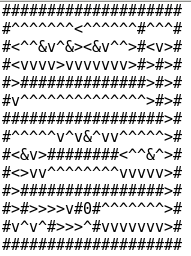
\includegraphics[scale=.5]{tst2-10.png}

\subsection{pacmaze-03-tricky.txt}

Formato do teste:

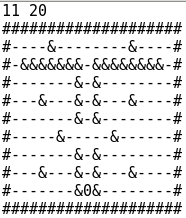
\includegraphics[scale=.5]{tst3-map.png}

$\alpha = 0.2$

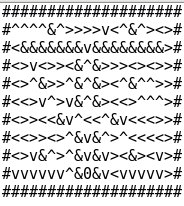
\includegraphics[scale=.5]{tst3-02.png}

$\alpha = 0.5$

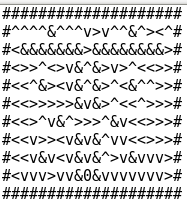
\includegraphics[scale=.5]{tst3-05.png}

$\alpha = 0.8$

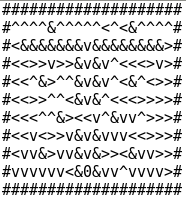
\includegraphics[scale=.5]{tst3-08.png}

$\alpha = 1.0$

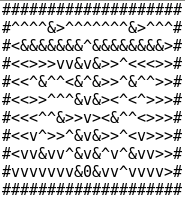
\includegraphics[scale=.5]{tst3-10.png}

Comparando os resultados dos testes, é notável o quanto o fator de aprendizado influencia na saída. Apesar de todos esses testes serem resultados intermediários, percebe-se que para taxas de aprendizado mais baixas, as decisões prioritárias são menos sólidas (em alguns momentos, andando em direção a recompensas mais baixas deliberadamente).

Isso não significa, porém, que uma taxa de aprendizado maior significa resultados melhores. Como é possível observar nas saídas com a taxa igual a 1, podem surgir tendências erradas para o agente e uma convergência prematura. Nesse caso, o agente ficaria preso às suas decisões erradas.

\subsection{Resultados após 100000 iterações}

Estes testes foram realizados com o valor da taxa de aprendizado 0.5.

pacmaze-01-tiny.txt - 

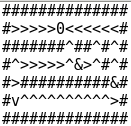
\includegraphics[scale=.5]{tst1-100k.png}

pacmaze-02-mid-sparse.txt -

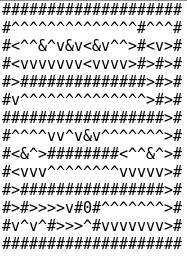
\includegraphics[scale=.5]{tst2-100k.png}

pacmaze-03-tricky.txt -

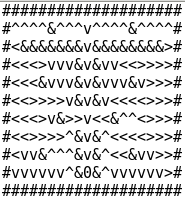
\includegraphics[scale=.5]{tst3-100k.png}

\section{Conclusão e possíveis melhorias}

O trabalho deixou bem evidente vários dilemas que surgem com a otimização de um espaço de estados parcialmente observável e, apesar de ser um método eficiente para este modelo de problema em particular, pode não ser o melhor para outras situações. O aprendizado por reforço implica que o agente precisa "errar" muito para abstrair uma política favorável e tornar-se viável. Se esse fosse o caso de um carro autónomo, por exemplo, significa que ele deve bater muito para finalmente aprender a dirigir. Apesar disso, há possíveis aplicações desse método para jogos eletrônicos, especialmente com ambientes não totalmente observáveis (ex. com \textit{fog of war}).

Um possível aprimoramento do programa, inclusive já sendo uma técnica aplicada nesse tipo de aprendizado e em outros (programação genética, inteligência de colônias, etc.) seria favorecer o \textit{exploitation} em vez do \textit{exploration} com o passar do tempo. No caso, isso seria feito incrementando gradualmente o valor de $\alpha$ com o passar do tempo.

Além disso, analogamente ao que ocorre em modelos de decisão de Markov para ambientes totalmente observáveis, caso os próximos estados além de $s'$ sejam observáveis, o valor deles pode ser considerado na atualização de $Q(s, a)$ (com o valor sendo descontado por $\gamma^n$). Isso ajudaria o agente a "enxergar mais um passo a frente" e pode auxiliar na convergência de estados mais distantes dos terminais, uma situação que ficou evidente neste trabalho.

Por fim, para esse problema, poderiam ter sido usados outros métodos como a programação genética (sendo a política ótima $\pi$ a função representada pelos indivíduos e a fitness representada pelo somatório das recompensas para agentes seguindo tal política).

\section{Referências}

\begin{enumerate}
	\item Russel, Norvig. \textit{Artificial Intelligence, A modern approach, 3rd edition}
\end{enumerate}

\end{document}